% Options for packages loaded elsewhere
\PassOptionsToPackage{unicode}{hyperref}
\PassOptionsToPackage{hyphens}{url}
%
\documentclass[
]{article}
\usepackage{amsmath,amssymb}
\usepackage{iftex}
\ifPDFTeX
  \usepackage[T1]{fontenc}
  \usepackage[utf8]{inputenc}
  \usepackage{textcomp} % provide euro and other symbols
\else % if luatex or xetex
  \usepackage{unicode-math} % this also loads fontspec
  \defaultfontfeatures{Scale=MatchLowercase}
  \defaultfontfeatures[\rmfamily]{Ligatures=TeX,Scale=1}
\fi
\usepackage{lmodern}
\ifPDFTeX\else
  % xetex/luatex font selection
    \setmainfont[]{Roboto}
    \setmonofont[]{Consolas}
\fi
% Use upquote if available, for straight quotes in verbatim environments
\IfFileExists{upquote.sty}{\usepackage{upquote}}{}
\IfFileExists{microtype.sty}{% use microtype if available
  \usepackage[]{microtype}
  \UseMicrotypeSet[protrusion]{basicmath} % disable protrusion for tt fonts
}{}
\makeatletter
\@ifundefined{KOMAClassName}{% if non-KOMA class
  \IfFileExists{parskip.sty}{%
    \usepackage{parskip}
  }{% else
    \setlength{\parindent}{0pt}
    \setlength{\parskip}{6pt plus 2pt minus 1pt}}
}{% if KOMA class
  \KOMAoptions{parskip=half}}
\makeatother
\usepackage{xcolor}
\usepackage[margin=1in]{geometry}
\usepackage{color}
\usepackage{fancyvrb}
\newcommand{\VerbBar}{|}
\newcommand{\VERB}{\Verb[commandchars=\\\{\}]}
\DefineVerbatimEnvironment{Highlighting}{Verbatim}{commandchars=\\\{\}}
% Add ',fontsize=\small' for more characters per line
\usepackage{framed}
\definecolor{shadecolor}{RGB}{248,248,248}
\newenvironment{Shaded}{\begin{snugshade}}{\end{snugshade}}
\newcommand{\AlertTok}[1]{\textcolor[rgb]{0.94,0.16,0.16}{#1}}
\newcommand{\AnnotationTok}[1]{\textcolor[rgb]{0.56,0.35,0.01}{\textbf{\textit{#1}}}}
\newcommand{\AttributeTok}[1]{\textcolor[rgb]{0.13,0.29,0.53}{#1}}
\newcommand{\BaseNTok}[1]{\textcolor[rgb]{0.00,0.00,0.81}{#1}}
\newcommand{\BuiltInTok}[1]{#1}
\newcommand{\CharTok}[1]{\textcolor[rgb]{0.31,0.60,0.02}{#1}}
\newcommand{\CommentTok}[1]{\textcolor[rgb]{0.56,0.35,0.01}{\textit{#1}}}
\newcommand{\CommentVarTok}[1]{\textcolor[rgb]{0.56,0.35,0.01}{\textbf{\textit{#1}}}}
\newcommand{\ConstantTok}[1]{\textcolor[rgb]{0.56,0.35,0.01}{#1}}
\newcommand{\ControlFlowTok}[1]{\textcolor[rgb]{0.13,0.29,0.53}{\textbf{#1}}}
\newcommand{\DataTypeTok}[1]{\textcolor[rgb]{0.13,0.29,0.53}{#1}}
\newcommand{\DecValTok}[1]{\textcolor[rgb]{0.00,0.00,0.81}{#1}}
\newcommand{\DocumentationTok}[1]{\textcolor[rgb]{0.56,0.35,0.01}{\textbf{\textit{#1}}}}
\newcommand{\ErrorTok}[1]{\textcolor[rgb]{0.64,0.00,0.00}{\textbf{#1}}}
\newcommand{\ExtensionTok}[1]{#1}
\newcommand{\FloatTok}[1]{\textcolor[rgb]{0.00,0.00,0.81}{#1}}
\newcommand{\FunctionTok}[1]{\textcolor[rgb]{0.13,0.29,0.53}{\textbf{#1}}}
\newcommand{\ImportTok}[1]{#1}
\newcommand{\InformationTok}[1]{\textcolor[rgb]{0.56,0.35,0.01}{\textbf{\textit{#1}}}}
\newcommand{\KeywordTok}[1]{\textcolor[rgb]{0.13,0.29,0.53}{\textbf{#1}}}
\newcommand{\NormalTok}[1]{#1}
\newcommand{\OperatorTok}[1]{\textcolor[rgb]{0.81,0.36,0.00}{\textbf{#1}}}
\newcommand{\OtherTok}[1]{\textcolor[rgb]{0.56,0.35,0.01}{#1}}
\newcommand{\PreprocessorTok}[1]{\textcolor[rgb]{0.56,0.35,0.01}{\textit{#1}}}
\newcommand{\RegionMarkerTok}[1]{#1}
\newcommand{\SpecialCharTok}[1]{\textcolor[rgb]{0.81,0.36,0.00}{\textbf{#1}}}
\newcommand{\SpecialStringTok}[1]{\textcolor[rgb]{0.31,0.60,0.02}{#1}}
\newcommand{\StringTok}[1]{\textcolor[rgb]{0.31,0.60,0.02}{#1}}
\newcommand{\VariableTok}[1]{\textcolor[rgb]{0.00,0.00,0.00}{#1}}
\newcommand{\VerbatimStringTok}[1]{\textcolor[rgb]{0.31,0.60,0.02}{#1}}
\newcommand{\WarningTok}[1]{\textcolor[rgb]{0.56,0.35,0.01}{\textbf{\textit{#1}}}}
\usepackage{graphicx}
\makeatletter
\def\maxwidth{\ifdim\Gin@nat@width>\linewidth\linewidth\else\Gin@nat@width\fi}
\def\maxheight{\ifdim\Gin@nat@height>\textheight\textheight\else\Gin@nat@height\fi}
\makeatother
% Scale images if necessary, so that they will not overflow the page
% margins by default, and it is still possible to overwrite the defaults
% using explicit options in \includegraphics[width, height, ...]{}
\setkeys{Gin}{width=\maxwidth,height=\maxheight,keepaspectratio}
% Set default figure placement to htbp
\makeatletter
\def\fps@figure{htbp}
\makeatother
\setlength{\emergencystretch}{3em} % prevent overfull lines
\providecommand{\tightlist}{%
  \setlength{\itemsep}{0pt}\setlength{\parskip}{0pt}}
\setcounter{secnumdepth}{-\maxdimen} % remove section numbering
\usepackage{fvextra}
\DefineVerbatimEnvironment{Highlighting}{Verbatim}{breaklines,commandchars=\\\{\}}
\ifLuaTeX
  \usepackage{selnolig}  % disable illegal ligatures
\fi
\usepackage{bookmark}
\IfFileExists{xurl.sty}{\usepackage{xurl}}{} % add URL line breaks if available
\urlstyle{same}
\hypersetup{
  pdftitle={Quantium Virtual Internship - Retail Strategy and Analytics - Task 1},
  hidelinks,
  pdfcreator={LaTeX via pandoc}}

\title{Quantium Virtual Internship - Retail Strategy and Analytics -
Task 1}
\author{}
\date{\vspace{-2.5em}}

\begin{document}
\maketitle

\begin{Shaded}
\begin{Highlighting}[]
\DocumentationTok{\#\#\#\# Example code to install packages}
\CommentTok{\#install.packages("data.table")}
\DocumentationTok{\#\#\#\# Load required libraries}
\FunctionTok{library}\NormalTok{(data.table)}
\end{Highlighting}
\end{Shaded}

\begin{verbatim}
## Warning: package 'data.table' was built under R version 4.3.2
\end{verbatim}

\begin{Shaded}
\begin{Highlighting}[]
\FunctionTok{library}\NormalTok{(ggplot2)}
\FunctionTok{library}\NormalTok{(ggmosaic)}
\end{Highlighting}
\end{Shaded}

\begin{verbatim}
## Warning: package 'ggmosaic' was built under R version 4.3.2
\end{verbatim}

\begin{Shaded}
\begin{Highlighting}[]
\FunctionTok{library}\NormalTok{(readr)}
\FunctionTok{library}\NormalTok{(readxl)}
\DocumentationTok{\#\#\#\# Point the filePath to where you have downloaded the datasets to and}
\DocumentationTok{\#\#\#\# assign the data files to data.tables}
\CommentTok{\# over to you! fill in the path to your working directory. If you are on a Windows machine, you will need to use forward slashes (/) instead of backshashes (\textbackslash{})}
\NormalTok{filePath }\OtherTok{\textless{}{-}} \StringTok{"C:/Users/bhuyl/OneDrive/Documents/filepath/"}
\NormalTok{transactionData }\OtherTok{\textless{}{-}} \FunctionTok{fread}\NormalTok{(}\FunctionTok{paste0}\NormalTok{(filePath,}\StringTok{"QVI\_transaction\_data.csv"}\NormalTok{))}
\NormalTok{customerData }\OtherTok{\textless{}{-}} \FunctionTok{fread}\NormalTok{(}\FunctionTok{paste0}\NormalTok{(filePath,}\StringTok{"QVI\_purchase\_behaviour.csv"}\NormalTok{))}
\end{Highlighting}
\end{Shaded}

\subsection{Exploratory data analysis}\label{exploratory-data-analysis}

The first step in any analysis is to first understand the data. Let's
take a look at each of the datasets provided. \#\#\# Examining
transaction data We can use \texttt{str()} to look at the format of each
column and see a sample of the data. As we have read in the dataset as a
\texttt{data.table} object, we can also run \texttt{transactionData} in
the console to see a sample of the data or use
\texttt{head(transactionData)} to look at the first 10 rows. Let's check
if columns we would expect to be numeric are in numeric form and date
columns are in date format.

\begin{Shaded}
\begin{Highlighting}[]
\DocumentationTok{\#\#\#\# Examine transaction data}
\CommentTok{\# Over to you! Examine the data using one or more of the methods described above.}
\FunctionTok{print}\NormalTok{(}\FunctionTok{str}\NormalTok{(transactionData))}
\end{Highlighting}
\end{Shaded}

\begin{verbatim}
## Classes 'data.table' and 'data.frame': 264836 obs. of 8 variables:
## $ DATE : int 43390 43599 43605 43329 43330 43604 43601 43601 43332 43330 ...
## $ STORE_NBR : int 1 1 1 2 2 4 4 4 5 7 ...
## $ LYLTY_CARD_NBR: int 1000 1307 1343 2373 2426 4074 4149 4196 5026 7150 ...
## $ TXN_ID : int 1 348 383 974 1038 2982 3333 3539 4525 6900 ...
## $ PROD_NBR : int 5 66 61 69 108 57 16 24 42 52 ...
## $ PROD_NAME : chr "Natural Chip Compny SeaSalt175g" "CCs Nacho Cheese 175g"
"Smiths Crinkle Cut Chips Chicken 170g" "Smiths Chip Thinly S/Cream&Onion 175g"
...
## $ PROD_QTY : int 2 3 2 5 3 1 1 1 1 2 ...
## $ TOT_SALES : num 6 6.3 2.9 15 13.8 5.1 5.7 3.6 3.9 7.2 ...
## - attr(*, ".internal.selfref")=<externalptr>
## NULL
\end{verbatim}

\begin{Shaded}
\begin{Highlighting}[]
\FunctionTok{print}\NormalTok{(}\FunctionTok{str}\NormalTok{(customerData))}
\end{Highlighting}
\end{Shaded}

\begin{verbatim}
## Classes 'data.table' and 'data.frame': 72637 obs. of 3 variables:
## $ LYLTY_CARD_NBR : int 1000 1002 1003 1004 1005 1007 1009 1010 1011 1012 ...
## $ LIFESTAGE : chr "YOUNG SINGLES/COUPLES" "YOUNG SINGLES/COUPLES" "YOUNG
FAMILIES" "OLDER SINGLES/COUPLES" ...
## $ PREMIUM_CUSTOMER: chr "Premium" "Mainstream" "Budget" "Mainstream" ...
## - attr(*, ".internal.selfref")=<externalptr>
## NULL
\end{verbatim}

We can see that the date column is in an integer format. Let's change
this to a date format.

\begin{Shaded}
\begin{Highlighting}[]
\DocumentationTok{\#\#\#\# Convert DATE column to a date format}
\DocumentationTok{\#\#\#\# A quick search online tells us that CSV and Excel integer dates begin on 30 Dec 1899}
\NormalTok{transactionData}\SpecialCharTok{$}\NormalTok{DATE }\OtherTok{\textless{}{-}} \FunctionTok{as.Date}\NormalTok{(transactionData}\SpecialCharTok{$}\NormalTok{DATE, }\AttributeTok{origin =} \StringTok{"1899{-}12{-}30"}\NormalTok{)}
\FunctionTok{head}\NormalTok{(transactionData}\SpecialCharTok{$}\NormalTok{DATE)}
\end{Highlighting}
\end{Shaded}

\begin{verbatim}
## [1] "2018-10-17" "2019-05-14" "2019-05-20" "2018-08-17" "2018-08-18"
## [6] "2019-05-19"
\end{verbatim}

We should check that we are looking at the right products by examining
PROD\_NAME.

\begin{Shaded}
\begin{Highlighting}[]
\DocumentationTok{\#\#\#\# Examine PROD\_NAME}
\CommentTok{\# Over to you! Generate a summary of the PROD\_NAME column.}
\FunctionTok{summary}\NormalTok{(transactionData[, PROD\_NAME])}
\end{Highlighting}
\end{Shaded}

\begin{verbatim}
##    Length     Class      Mode 
##    264836 character character
\end{verbatim}

\begin{Shaded}
\begin{Highlighting}[]
\FunctionTok{table}\NormalTok{(transactionData[, PROD\_NAME])}
\end{Highlighting}
\end{Shaded}

\begin{verbatim}
## 
##                        Burger Rings 220g 
##                                     1564 
##                 CCs Nacho Cheese    175g 
##                                     1498 
##                        CCs Original 175g 
##                                     1514 
##                 CCs Tasty Cheese    175g 
##                                     1539 
##           Cheetos Chs & Bacon Balls 190g 
##                                     1479 
##                       Cheetos Puffs 165g 
##                                     1448 
##                     Cheezels Cheese 330g 
##                                     3149 
##                 Cheezels Cheese Box 125g 
##                                     1454 
##           Cobs Popd Sea Salt  Chips 110g 
##                                     3265 
##   Cobs Popd Sour Crm  &Chives Chips 110g 
##                                     3159 
## Cobs Popd Swt/Chlli &Sr/Cream Chips 110g 
##                                     3269 
##         Dorito Corn Chp     Supreme 380g 
##                                     3185 
##         Doritos Cheese      Supreme 330g 
##                                     3052 
##  Doritos Corn Chip Mexican Jalapeno 150g 
##                                     3204 
##  Doritos Corn Chip Southern Chicken 150g 
##                                     3172 
##  Doritos Corn Chips  Cheese Supreme 170g 
##                                     3217 
##    Doritos Corn Chips  Nacho Cheese 170g 
##                                     3160 
##        Doritos Corn Chips  Original 170g 
##                                     3121 
##                 Doritos Mexicana    170g 
##                                     3115 
##          Doritos Salsa       Medium 300g 
##                                     1449 
##                 Doritos Salsa Mild  300g 
##                                     1472 
##           French Fries Potato Chips 175g 
##                                     1418 
##    Grain Waves         Sweet Chilli 210g 
##                                     3167 
##    Grain Waves Sour    Cream&Chives 210G 
##                                     3105 
##    GrnWves Plus Btroot & Chilli Jam 180g 
##                                     1468 
##  Infuzions BBQ Rib   Prawn Crackers 110g 
##                                     3174 
##  Infuzions Mango     Chutny Papadums 70g 
##                                     1507 
## Infuzions SourCream&Herbs Veg Strws 110g 
##                                     3134 
## Infuzions Thai SweetChili PotatoMix 110g 
##                                     3242 
##   Infzns Crn Crnchers Tangy Gcamole 110g 
##                                     3144 
##             Kettle 135g Swt Pot Sea Salt 
##                                     3257 
##                       Kettle Chilli 175g 
##                                     3038 
##         Kettle Honey Soy    Chicken 175g 
##                                     3148 
##   Kettle Mozzarella   Basil & Pesto 175g 
##                                     3304 
##                     Kettle Original 175g 
##                                     3159 
##     Kettle Sea Salt     And Vinegar 175g 
##                                     3173 
##       Kettle Sensations   BBQ&Maple 150g 
##                                     3083 
## Kettle Sensations   Camembert & Fig 150g 
##                                     3219 
##    Kettle Sensations   Siracha Lime 150g 
##                                     3127 
##  Kettle Sweet Chilli And Sour Cream 175g 
##                                     3200 
##  Kettle Tortilla ChpsBtroot&Ricotta 150g 
##                                     3146 
##     Kettle Tortilla ChpsFeta&Garlic 150g 
##                                     3138 
## Kettle Tortilla ChpsHny&Jlpno Chili 150g 
##                                     3296 
##   Natural Chip        Compny SeaSalt175g 
##                                     1468 
##  Natural Chip Co     Tmato Hrb&Spce 175g 
##                                     1572 
##   Natural ChipCo      Hony Soy Chckn175g 
##                                     1460 
##   Natural ChipCo Sea  Salt & Vinegr 175g 
##                                     1550 
##   NCC Sour Cream &    Garden Chives 175g 
##                                     1419 
## Old El Paso Salsa   Dip Chnky Tom Ht300g 
##                                     3125 
##  Old El Paso Salsa   Dip Tomato Med 300g 
##                                     3114 
## Old El Paso Salsa   Dip Tomato Mild 300g 
##                                     3085 
##                 Pringles Barbeque   134g 
##                                     3210 
##      Pringles Chicken    Salt Crips 134g 
##                                     3104 
##         Pringles Mystery    Flavour 134g 
##                                     3114 
##          Pringles Original   Crisps 134g 
##                                     3157 
##                 Pringles Slt Vingar 134g 
##                                     3095 
##           Pringles SourCream  Onion 134g 
##                                     3162 
##         Pringles Sthrn FriedChicken 134g 
##                                     3083 
##             Pringles Sweet&Spcy BBQ 134g 
##                                     3177 
##    Red Rock Deli Chikn&Garlic Aioli 150g 
##                                     1434 
##  Red Rock Deli Sp    Salt & Truffle 150G 
##                                     1498 
## Red Rock Deli SR    Salsa & Mzzrlla 150g 
##                                     1458 
##     Red Rock Deli Thai  Chilli&Lime 150g 
##                                     1495 
##         RRD Chilli&         Coconut 150g 
##                                     1506 
##         RRD Honey Soy       Chicken 165g 
##                                     1513 
##                 RRD Lime & Pepper   165g 
##                                     1473 
##                 RRD Pc Sea Salt     165g 
##                                     1431 
##                 RRD Salt & Vinegar  165g 
##                                     1474 
##      RRD SR Slow Rst     Pork Belly 150g 
##                                     1526 
##     RRD Steak &         Chimuchurri 150g 
##                                     1455 
##      RRD Sweet Chilli &  Sour Cream 165g 
##                                     1516 
##       Smith Crinkle Cut   Bolognese 150g 
##                                     1451 
##    Smith Crinkle Cut   Mac N Cheese 150g 
##                                     1512 
##    Smiths Chip Thinly  Cut Original 175g 
##                                     1614 
##   Smiths Chip Thinly  CutSalt/Vinegr175g 
##                                     1440 
##   Smiths Chip Thinly  S/Cream&Onion 175g 
##                                     1473 
##        Smiths Crinkle      Original 330g 
##                                     3142 
## Smiths Crinkle Chips Salt & Vinegar 330g 
##                                     3197 
##  Smiths Crinkle Cut  Chips Barbecue 170g 
##                                     1489 
##   Smiths Crinkle Cut  Chips Chicken 170g 
##                                     1484 
##  Smiths Crinkle Cut  Chips Chs&Onion170g 
##                                     1481 
##  Smiths Crinkle Cut  Chips Original 170g 
##                                     1461 
## Smiths Crinkle Cut  French OnionDip 150g 
##                                     1438 
##  Smiths Crinkle Cut  Salt & Vinegar 170g 
##                                     1455 
##      Smiths Crinkle Cut  Snag&Sauce 150g 
##                                     1503 
##    Smiths Crinkle Cut  Tomato Salsa 150g 
##                                     1470 
##   Smiths Crnkle Chip  Orgnl Big Bag 380g 
##                                     3233 
## Smiths Thinly       Swt Chli&S/Cream175G 
##                                     1461 
##   Smiths Thinly Cut   Roast Chicken 175g 
##                                     1519 
##     Snbts Whlgrn Crisps Cheddr&Mstrd 90g 
##                                     1576 
## Sunbites Whlegrn    Crisps Frch/Onin 90g 
##                                     1432 
##   Thins Chips         Originl saltd 175g 
##                                     1441 
##           Thins Chips Light&  Tangy 175g 
##                                     3188 
##         Thins Chips Salt &  Vinegar 175g 
##                                     3103 
##         Thins Chips Seasonedchicken 175g 
##                                     3114 
##     Thins Potato Chips  Hot & Spicy 175g 
##                                     3229 
##          Tostitos Lightly    Salted 175g 
##                                     3074 
##        Tostitos Smoked     Chipotle 175g 
##                                     3145 
##            Tostitos Splash Of  Lime 175g 
##                                     3252 
##                 Twisties Cheese     270g 
##                                     3115 
##          Twisties Cheese     Burger 250g 
##                                     3169 
##                     Twisties Chicken270g 
##                                     3170 
##   Tyrrells Crisps     Ched & Chives 165g 
##                                     3268 
##  Tyrrells Crisps     Lightly Salted 165g 
##                                     3174 
##           Woolworths Cheese   Rings 190g 
##                                     1516 
##           Woolworths Medium   Salsa 300g 
##                                     1430 
##           Woolworths Mild     Salsa 300g 
##                                     1491 
##         WW Crinkle Cut      Chicken 175g 
##                                     1467 
##        WW Crinkle Cut      Original 175g 
##                                     1410 
##        WW D/Style Chip     Sea Salt 200g 
##                                     1469 
##           WW Original Corn    Chips 200g 
##                                     1495 
##           WW Original Stacked Chips 160g 
##                                     1487 
##   WW Sour Cream &OnionStacked Chips 160g 
##                                     1483 
##      WW Supreme Cheese   Corn Chips 200g 
##                                     1509
\end{verbatim}

Looks like we are definitely looking at potato chips but how can we
check that these are all chips? We can do some basic text analysis by
summarising the individual words in the product name.

\begin{Shaded}
\begin{Highlighting}[]
\DocumentationTok{\#\#\#\# Examine the words in PROD\_NAME to see if there are any incorrect entries}
\DocumentationTok{\#\#\#\# such as products that are not chips}
\NormalTok{productWords }\OtherTok{\textless{}{-}} \FunctionTok{data.table}\NormalTok{(}\FunctionTok{unlist}\NormalTok{(}\FunctionTok{strsplit}\NormalTok{(}\FunctionTok{unique}\NormalTok{(transactionData[, PROD\_NAME]), }\StringTok{"}
\StringTok{"}\NormalTok{)))}
\FunctionTok{setnames}\NormalTok{(productWords, }\StringTok{\textquotesingle{}words\textquotesingle{}}\NormalTok{)}
\end{Highlighting}
\end{Shaded}

As we are only interested in words that will tell us if the product is
chips or not, let's remove all words with digits and special characters
such as `\&' from our set of product words. We can do this using
\texttt{grepl()}.

\begin{Shaded}
\begin{Highlighting}[]
\FunctionTok{library}\NormalTok{(stringr)}
\FunctionTok{library}\NormalTok{(stringi)}
\CommentTok{\# Over to you! Remove digits, and special characters, and then sort the distinct words by frequency of occurrence.}
\DocumentationTok{\#\#\#\# Removing digits}
\NormalTok{productWords}\SpecialCharTok{$}\NormalTok{words }\OtherTok{\textless{}{-}} \FunctionTok{str\_replace\_all}\NormalTok{(productWords}\SpecialCharTok{$}\NormalTok{words, }\StringTok{"[[:punct:]]"}\NormalTok{,}\StringTok{" "}\NormalTok{)}
\DocumentationTok{\#\#\#\# Removing special characters}
\NormalTok{productWords}\SpecialCharTok{$}\NormalTok{words }\OtherTok{\textless{}{-}} \FunctionTok{str\_replace\_all}\NormalTok{(productWords}\SpecialCharTok{$}\NormalTok{words, }\StringTok{"[0{-}9]"}\NormalTok{, }\StringTok{" "}\NormalTok{)}
\NormalTok{productWords}\SpecialCharTok{$}\NormalTok{words }\OtherTok{\textless{}{-}} \FunctionTok{str\_replace\_all}\NormalTok{(productWords}\SpecialCharTok{$}\NormalTok{words, }\StringTok{"[gG]"}\NormalTok{, }\StringTok{" "}\NormalTok{)}
\DocumentationTok{\#\#\#\# Let\textquotesingle{}s look at the most common words by counting the number of times a word appears and}
\NormalTok{wordsSep }\OtherTok{\textless{}{-}} \FunctionTok{strsplit}\NormalTok{(productWords}\SpecialCharTok{$}\NormalTok{words, }\StringTok{" "}\NormalTok{)}
\NormalTok{words.freq }\OtherTok{\textless{}{-}} \FunctionTok{table}\NormalTok{(}\FunctionTok{unlist}\NormalTok{(wordsSep))}
\DocumentationTok{\#\#\#\# sorting them by this frequency in order of highest to lowest frequency}
\NormalTok{words.freq }\OtherTok{\textless{}{-}} \FunctionTok{as.data.frame}\NormalTok{(words.freq)}
\NormalTok{words.freq }\OtherTok{\textless{}{-}}\NormalTok{ words.freq[}\FunctionTok{order}\NormalTok{(words.freq}\SpecialCharTok{$}\NormalTok{Freq, }\AttributeTok{decreasing =}\NormalTok{ T),]}
\NormalTok{words.freq}
\end{Highlighting}
\end{Shaded}

\begin{verbatim}
##                Var1 Freq
## 1                    732
## 37            Chips   21
## 164          Smiths   16
## 55          Crinkle   14
## 62              Cut   14
## 92           Kettle   13
## 26           Cheese   12
## 152            Salt   12
## 122             Ori   11
## 85             inal   10
## 34             Chip    9
## 68          Doritos    9
## 151           Salsa    9
## 29          Chicken    8
## 52             Corn    8
## 54            Cream    8
## 93              les    8
## 135            Prin    8
## 147             RRD    8
## 32           Chilli    7
## 204            Vine    7
## 209              WW    7
## 4                ar    6
## 156             Sea    6
## 168            Sour    6
## 57           Crisps    5
## 192          Thinly    5
## 193           Thins    5
## 38           Chives    4
## 65             Deli    4
## 86        Infuzions    4
## 95             Lime    4
## 110         Natural    4
## 139             Red    4
## 146            Rock    4
## 185         Supreme    4
## 186           Sweet    4
## 13              BBQ    3
## 22              CCs    3
## 49             Cobs    3
## 66              Dip    3
## 69               El    3
## 94               Li    3
## 103            Mild    3
## 116             Old    3
## 118           Onion    3
## 124            Paso    3
## 129            Popd    3
## 159      Sensations    3
## 171             Soy    3
## 188             Swt    3
## 196          Tomato    3
## 197        Tortilla    3
## 198        Tostitos    3
## 200        Twisties    3
## 208      Woolworths    3
## 3               And    2
## 6             arlic    2
## 19              Bur    2
## 27          Cheetos    2
## 28         Cheezels    2
## 35           ChipCo    2
## 46              Chs    2
## 70               er    2
## 74           French    2
## 78            Honey    2
## 84             htly    2
## 100          Medium    2
## 109           Nacho    2
## 132          Potato    2
## 137               r    2
## 138            rain    2
## 142             Rin    2
## 143              rn    2
## 149               s    2
## 150               S    2
## 154          Salted    2
## 163           Smith    2
## 169       SourCream    2
## 178              SR    2
## 189             Tan    2
## 191            Thai    2
## 201        Tyrrells    2
## 205           Waves    2
## 210               y    2
## 2             Aioli    1
## 5             arden    1
## 7                Ba    1
## 8             Bacon    1
## 9             Balls    1
## 10         Barbecue    1
## 11         Barbeque    1
## 12            Basil    1
## 14            Belly    1
## 15               Bi    1
## 16             Bolo    1
## 17              Box    1
## 18           Btroot    1
## 20        Camembert    1
## 21           camole    1
## 23            Chckn    1
## 24             Ched    1
## 25           Cheddr    1
## 30            Chikn    1
## 31            Chili    1
## 33      Chimuchurri    1
## 36         Chipotle    1
## 39             Chli    1
## 40            Chlli    1
## 41            Chnky    1
## 42              Chp    1
## 43       ChpsBtroot    1
## 44         ChpsFeta    1
## 45          ChpsHny    1
## 47           Chutny    1
## 48               Co    1
## 50          Coconut    1
## 51           Compny    1
## 53         Crackers    1
## 56            Crips    1
## 58              Crm    1
## 59              Crn    1
## 60         Crnchers    1
## 61           Crnkle    1
## 63          CutSalt    1
## 64                D    1
## 67           Dorito    1
## 71               Fi    1
## 72          Flavour    1
## 73             Frch    1
## 75     FriedChicken    1
## 76            Fries    1
## 77            Herbs    1
## 79             Hony    1
## 80              Hot    1
## 81              Hrb    1
## 82               ht    1
## 83               Ht    1
## 87           Infzns    1
## 88              inl    1
## 89         Jalapeno    1
## 90              Jam    1
## 91            Jlpno    1
## 96              Mac    1
## 97              Man    1
## 98            Maple    1
## 99              Med    1
## 101         Mexican    1
## 102        Mexicana    1
## 104      Mozzarella    1
## 105           Mstrd    1
## 106         Mystery    1
## 107         Mzzrlla    1
## 108               N    1
## 111             NCC    1
## 112            nese    1
## 113              nl    1
## 114               o    1
## 115              Of    1
## 117            Onin    1
## 119        OnionDip    1
## 120    OnionStacked    1
## 121              Or    1
## 123        Papadums    1
## 125              Pc    1
## 126          Pepper    1
## 127           Pesto    1
## 128            Plus    1
## 130            Pork    1
## 131             Pot    1
## 133       PotatoMix    1
## 134           Prawn    1
## 136           Puffs    1
## 140             Rib    1
## 141         Ricotta    1
## 144          rnWves    1
## 145           Roast    1
## 148             Rst    1
## 153           saltd    1
## 155           Sauce    1
## 157         SeaSalt    1
## 158 Seasonedchicken    1
## 160         Siracha    1
## 161            Slow    1
## 162             Slt    1
## 165          Smoked    1
## 166             Sna    1
## 167           Snbts    1
## 170        Southern    1
## 172              Sp    1
## 173            Spce    1
## 174            Spcy    1
## 175           Spicy    1
## 176          Splash    1
## 177              Sr    1
## 179         Stacked    1
## 180           Steak    1
## 181           Sthrn    1
## 182           Strws    1
## 183           Style    1
## 184        Sunbites    1
## 187      SweetChili    1
## 190           Tasty    1
## 194           Tmato    1
## 195             Tom    1
## 199         Truffle    1
## 202              Ve    1
## 203             Vin    1
## 206             Whl    1
## 207            Whle    1
\end{verbatim}

There are salsa products in the dataset but we are only interested in
the chips category, so let's remove these.

\begin{Shaded}
\begin{Highlighting}[]
\DocumentationTok{\#\#\#\# Remove salsa products}
\NormalTok{transactionData[, SALSA }\SpecialCharTok{:=} \FunctionTok{grepl}\NormalTok{(}\StringTok{"salsa"}\NormalTok{, }\FunctionTok{tolower}\NormalTok{(PROD\_NAME))]}
\NormalTok{transactionData }\OtherTok{\textless{}{-}}\NormalTok{ transactionData[SALSA }\SpecialCharTok{==} \ConstantTok{FALSE}\NormalTok{, ][, SALSA }\SpecialCharTok{:=} \ConstantTok{NULL}\NormalTok{]}
\end{Highlighting}
\end{Shaded}

Next, we can use \texttt{summary()} to check summary statistics such as
mean, min and max values for each feature to see if there are any
obvious outliers in the data and if there are any nulls in any of the
columns (\texttt{NA\textquotesingle{}s\ :\ number\ of\ nulls} will
appear in the output if there are any nulls).

\begin{Shaded}
\begin{Highlighting}[]
\DocumentationTok{\#\#\#\# Summarise the data to check for nulls and possible outliers}
\CommentTok{\# Over to you!}
\FunctionTok{summary}\NormalTok{(transactionData)}
\end{Highlighting}
\end{Shaded}

\begin{verbatim}
##       DATE              STORE_NBR     LYLTY_CARD_NBR        TXN_ID       
##  Min.   :2018-07-01   Min.   :  1.0   Min.   :   1000   Min.   :      1  
##  1st Qu.:2018-09-30   1st Qu.: 70.0   1st Qu.:  70015   1st Qu.:  67569  
##  Median :2018-12-30   Median :130.0   Median : 130367   Median : 135183  
##  Mean   :2018-12-30   Mean   :135.1   Mean   : 135531   Mean   : 135131  
##  3rd Qu.:2019-03-31   3rd Qu.:203.0   3rd Qu.: 203084   3rd Qu.: 202654  
##  Max.   :2019-06-30   Max.   :272.0   Max.   :2373711   Max.   :2415841  
##     PROD_NBR       PROD_NAME            PROD_QTY         TOT_SALES      
##  Min.   :  1.00   Length:246742      Min.   :  1.000   Min.   :  1.700  
##  1st Qu.: 26.00   Class :character   1st Qu.:  2.000   1st Qu.:  5.800  
##  Median : 53.00   Mode  :character   Median :  2.000   Median :  7.400  
##  Mean   : 56.35                      Mean   :  1.908   Mean   :  7.321  
##  3rd Qu.: 87.00                      3rd Qu.:  2.000   3rd Qu.:  8.800  
##  Max.   :114.00                      Max.   :200.000   Max.   :650.000
\end{verbatim}

There are no nulls in the columns but product quantity appears to have
an outlier which we should investigate further. Let's investigate
further the case where 200 packets of chips are bought in one
transaction.

\begin{Shaded}
\begin{Highlighting}[]
\FunctionTok{library}\NormalTok{(tidyverse)}
\end{Highlighting}
\end{Shaded}

\begin{verbatim}
## Warning: package 'tidyr' was built under R version 4.3.2
\end{verbatim}

\begin{verbatim}
## -- Attaching core tidyverse packages ------------------------ tidyverse 2.0.0 --
## v dplyr     1.1.3     v purrr     1.0.2
## v forcats   1.0.0     v tibble    3.2.1
## v lubridate 1.9.2     v tidyr     1.3.0
## -- Conflicts ------------------------------------------ tidyverse_conflicts() --
## x dplyr::between()     masks data.table::between()
## x dplyr::filter()      masks stats::filter()
## x dplyr::first()       masks data.table::first()
## x lubridate::hour()    masks data.table::hour()
## x lubridate::isoweek() masks data.table::isoweek()
## x dplyr::lag()         masks stats::lag()
## x dplyr::last()        masks data.table::last()
## x lubridate::mday()    masks data.table::mday()
## x lubridate::minute()  masks data.table::minute()
## x lubridate::month()   masks data.table::month()
## x lubridate::quarter() masks data.table::quarter()
## x lubridate::second()  masks data.table::second()
## x purrr::transpose()   masks data.table::transpose()
## x lubridate::wday()    masks data.table::wday()
## x lubridate::week()    masks data.table::week()
## x lubridate::yday()    masks data.table::yday()
## x lubridate::year()    masks data.table::year()
## i Use the conflicted package (<http://conflicted.r-lib.org/>) to force all conflicts to become errors
\end{verbatim}

\begin{Shaded}
\begin{Highlighting}[]
\FunctionTok{library}\NormalTok{(dplyr)}
\DocumentationTok{\#\#\#\# Filter the dataset to find the outlier}
\CommentTok{\# Over to you! Use a filter to examine the transactions in question.}
\end{Highlighting}
\end{Shaded}

\begin{Shaded}
\begin{Highlighting}[]
\NormalTok{prod\_qty\_200 }\OtherTok{\textless{}{-}}\NormalTok{ transactionData }\SpecialCharTok{\%\textgreater{}\%} \FunctionTok{filter}\NormalTok{(PROD\_QTY}\SpecialCharTok{==}\DecValTok{200}\NormalTok{)}
\NormalTok{check\_for\_the\_same }\OtherTok{\textless{}{-}}\NormalTok{ transactionData }\SpecialCharTok{\%\textgreater{}\%} \FunctionTok{filter}\NormalTok{(transactionData}\SpecialCharTok{$}\NormalTok{LYLTY\_CARD\_NBR }\SpecialCharTok{==} \DecValTok{22600}\NormalTok{)}
\end{Highlighting}
\end{Shaded}

There are two transactions where 200 packets of chips are bought in one
transaction and both of these transactions were by the same customer.

\begin{Shaded}
\begin{Highlighting}[]
\DocumentationTok{\#\#\#\# Let\textquotesingle{}s see if the customer has had other transactions}
\CommentTok{\# Over to you! Use a filter to see what other transactions that customer made.}
\NormalTok{transactionData }\OtherTok{\textless{}{-}}\NormalTok{ transactionData[}\SpecialCharTok{!}\NormalTok{(transactionData}\SpecialCharTok{$}\NormalTok{LYLTY\_CARD\_NBR }\SpecialCharTok{==} \DecValTok{22600}\NormalTok{)]}
\FunctionTok{summary}\NormalTok{(transactionData)}
\end{Highlighting}
\end{Shaded}

\begin{verbatim}
##       DATE              STORE_NBR     LYLTY_CARD_NBR        TXN_ID       
##  Min.   :2018-07-01   Min.   :  1.0   Min.   :   1000   Min.   :      1  
##  1st Qu.:2018-09-30   1st Qu.: 70.0   1st Qu.:  70015   1st Qu.:  67569  
##  Median :2018-12-30   Median :130.0   Median : 130367   Median : 135183  
##  Mean   :2018-12-30   Mean   :135.1   Mean   : 135531   Mean   : 135131  
##  3rd Qu.:2019-03-31   3rd Qu.:203.0   3rd Qu.: 203084   3rd Qu.: 202654  
##  Max.   :2019-06-30   Max.   :272.0   Max.   :2373711   Max.   :2415841  
##     PROD_NBR       PROD_NAME            PROD_QTY         TOT_SALES      
##  Min.   :  1.00   Length:246742      Min.   :  1.000   Min.   :  1.700  
##  1st Qu.: 26.00   Class :character   1st Qu.:  2.000   1st Qu.:  5.800  
##  Median : 53.00   Mode  :character   Median :  2.000   Median :  7.400  
##  Mean   : 56.35                      Mean   :  1.908   Mean   :  7.321  
##  3rd Qu.: 87.00                      3rd Qu.:  2.000   3rd Qu.:  8.800  
##  Max.   :114.00                      Max.   :200.000   Max.   :650.000
\end{verbatim}

It looks like this customer has only had the two transactions over the
year and is not an ordinary retail customer. The customer might be
buying chips for commercial purposes instead. We'll remove this loyalty
card number from further analysis.

\begin{Shaded}
\begin{Highlighting}[]
\DocumentationTok{\#\#\#\# Filter out the customer based on the loyalty card number}
\CommentTok{\# Over to you!}
\DocumentationTok{\#\#\#\# Re{-}examine transaction data}
\CommentTok{\# Over to you!}
\end{Highlighting}
\end{Shaded}

That's better. Now, let's look at the number of transaction lines over
time to see if there are any obvious data issues such as missing data.

\begin{Shaded}
\begin{Highlighting}[]
\DocumentationTok{\#\#\#\# Count the number of transactions by date}
\CommentTok{\# Over to you! Create a summary of transaction count by date.}
\DocumentationTok{\#\#\#\# Count the number of transactions by date}
\NormalTok{countByDate }\OtherTok{\textless{}{-}} \FunctionTok{count}\NormalTok{(transactionData, transactionData}\SpecialCharTok{$}\NormalTok{DATE)}
\NormalTok{countByDate}
\end{Highlighting}
\end{Shaded}

\begin{verbatim}
##      transactionData$DATE     n
##                    <Date> <int>
##   1:           2018-07-01   663
##   2:           2018-07-02   650
##   3:           2018-07-03   674
##   4:           2018-07-04   669
##   5:           2018-07-05   660
##  ---                           
## 360:           2019-06-26   657
## 361:           2019-06-27   669
## 362:           2019-06-28   673
## 363:           2019-06-29   703
## 364:           2019-06-30   704
\end{verbatim}

There's only 364 rows, meaning only 364 dates which indicates a missing
date. Let's create a sequence of dates from 1 Jul 2018 to 30 Jun 2019
and use this to create a chart of number of transactions over time to
find the missing date.

\begin{Shaded}
\begin{Highlighting}[]
\NormalTok{transactions\_by\_day }\OtherTok{\textless{}{-}}\NormalTok{ transactionData[}\FunctionTok{order}\NormalTok{(DATE), ]}
\end{Highlighting}
\end{Shaded}

\begin{Shaded}
\begin{Highlighting}[]
\DocumentationTok{\#\#\#\# Create a sequence of dates and join this the count of transactions by date}
\CommentTok{\# Over to you {-} create a column of dates that includes every day from 1 Jul 2018 to 30 Jun 2019, and join it onto the data to fill in the missing day.}
\DocumentationTok{\#\#\#\# Setting plot themes to format graphs}
\FunctionTok{theme\_set}\NormalTok{(}\FunctionTok{theme\_bw}\NormalTok{())}
\FunctionTok{theme\_update}\NormalTok{(}\AttributeTok{plot.title =} \FunctionTok{element\_text}\NormalTok{(}\AttributeTok{hjust =} \FloatTok{0.5}\NormalTok{))}
\DocumentationTok{\#\#\#\# Plot transactions over time}
\FunctionTok{ggplot}\NormalTok{(countByDate, }\FunctionTok{aes}\NormalTok{(}\AttributeTok{x =}\NormalTok{ countByDate}\SpecialCharTok{$}\StringTok{\textasciigrave{}}\AttributeTok{transactionData$DATE}\StringTok{\textasciigrave{}}\NormalTok{, }\AttributeTok{y =}\NormalTok{ countByDate}\SpecialCharTok{$}\NormalTok{n)) }\SpecialCharTok{+}
 \FunctionTok{geom\_line}\NormalTok{() }\SpecialCharTok{+}
 \FunctionTok{labs}\NormalTok{(}\AttributeTok{x =} \StringTok{"Day"}\NormalTok{, }\AttributeTok{y =} \StringTok{"Number of transactions"}\NormalTok{, }\AttributeTok{title =} \StringTok{"Transactions over time"}\NormalTok{) }\SpecialCharTok{+}
 \FunctionTok{scale\_x\_date}\NormalTok{(}\AttributeTok{breaks =} \StringTok{"1 month"}\NormalTok{) }\SpecialCharTok{+}
 \FunctionTok{theme}\NormalTok{(}\AttributeTok{axis.text.x =} \FunctionTok{element\_text}\NormalTok{(}\AttributeTok{angle =} \DecValTok{90}\NormalTok{, }\AttributeTok{vjust =} \FloatTok{0.5}\NormalTok{))}
\end{Highlighting}
\end{Shaded}

\begin{center}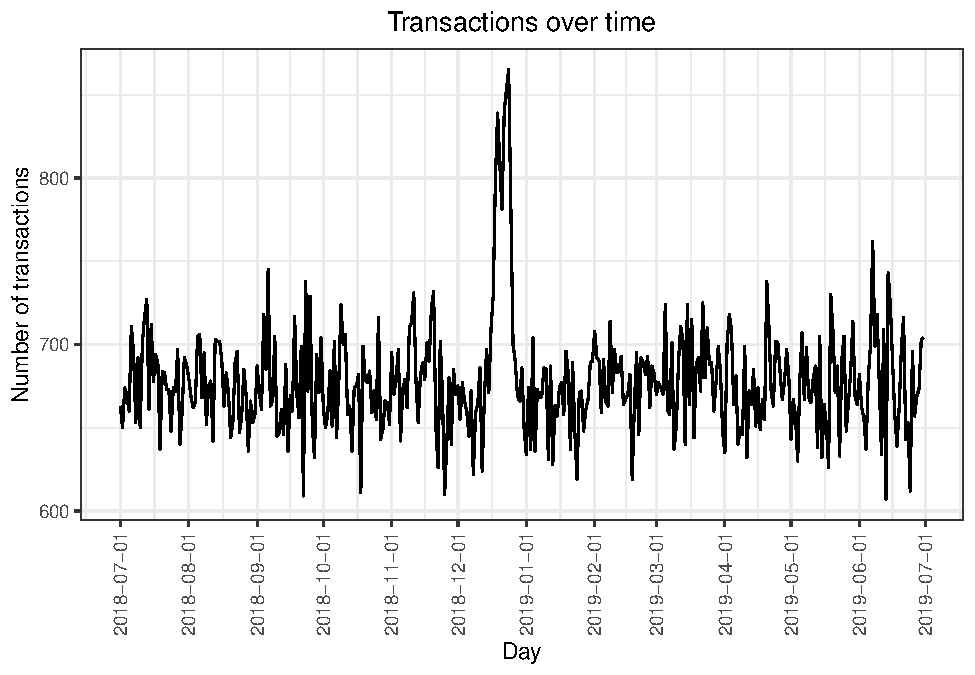
\includegraphics{InsideSherpa_Task1_files/figure-latex/unnamed-chunk-10-1} \end{center}

We can see that there is an increase in purchases in December and a
break in late December. Let's zoom in on this.

\begin{Shaded}
\begin{Highlighting}[]
\DocumentationTok{\#\#\#\# Filter to December and look at individual days}
\CommentTok{\# Over to you {-} recreate the chart above zoomed in to the relevant dates.}
\NormalTok{filterData }\OtherTok{\textless{}{-}}\NormalTok{ countByDate[countByDate}\SpecialCharTok{$}\StringTok{\textasciigrave{}}\AttributeTok{transactionData$DATE}\StringTok{\textasciigrave{}} \SpecialCharTok{\textgreater{}=} \StringTok{"2018{-}12{-}01"} \SpecialCharTok{\&}\NormalTok{ countByDate}\SpecialCharTok{$}\StringTok{\textasciigrave{}}\AttributeTok{transactionData$DATE}\StringTok{\textasciigrave{}} \SpecialCharTok{\textless{}=} \StringTok{"2018{-}12{-}31"}\NormalTok{]}
\FunctionTok{ggplot}\NormalTok{(filterData, }\FunctionTok{aes}\NormalTok{(}\AttributeTok{x =}\NormalTok{ filterData}\SpecialCharTok{$}\StringTok{\textasciigrave{}}\AttributeTok{transactionData$DATE}\StringTok{\textasciigrave{}}\NormalTok{, }\AttributeTok{y =}\NormalTok{ filterData}\SpecialCharTok{$}\NormalTok{n)) }\SpecialCharTok{+} 
  \FunctionTok{geom\_line}\NormalTok{() }\SpecialCharTok{+} 
  \FunctionTok{labs}\NormalTok{(}\AttributeTok{x =} \StringTok{"Day"}\NormalTok{, }\AttributeTok{y =} \StringTok{"Number of transactions"}\NormalTok{, }\AttributeTok{title =} \StringTok{"Transactions in December"}\NormalTok{) }\SpecialCharTok{+}
  \FunctionTok{scale\_x\_date}\NormalTok{(}\AttributeTok{breaks =} \StringTok{"1 day"}\NormalTok{) }\SpecialCharTok{+}
  \FunctionTok{theme}\NormalTok{(}\AttributeTok{axis.text.x =} \FunctionTok{element\_text}\NormalTok{(}\AttributeTok{angle =} \DecValTok{90}\NormalTok{, }\AttributeTok{vjust =} \FloatTok{0.5}\NormalTok{))}
\end{Highlighting}
\end{Shaded}

\begin{center}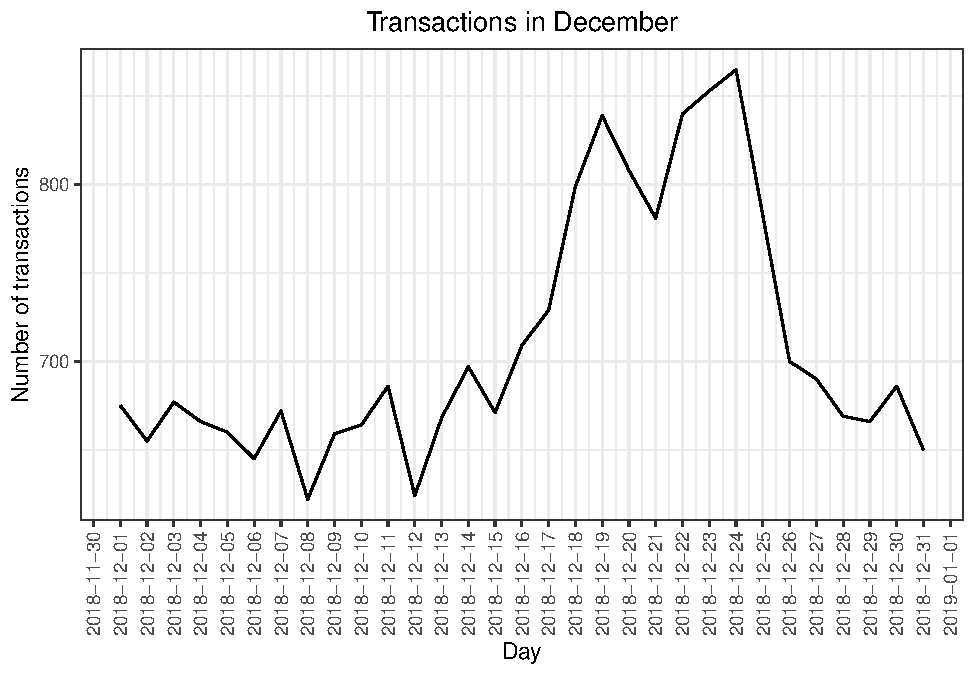
\includegraphics{InsideSherpa_Task1_files/figure-latex/unnamed-chunk-11-1} \end{center}

We can see that the increase in sales occurs in the lead-up to Christmas
and that there are zero sales on Christmas day itself. This is due to
shops being closed on Christmas day. Now that we are satisfied that the
data no longer has outliers, we can move on to creating other features
such as brand of chips or pack size from PROD\_NAME. We will start with
pack size.

\begin{Shaded}
\begin{Highlighting}[]
\DocumentationTok{\#\#\#\# Pack size}
\DocumentationTok{\#\#\#\# We can work this out by taking the digits that are in PROD\_NAME}
\NormalTok{transactionData[, PACK\_SIZE }\SpecialCharTok{:=} \FunctionTok{parse\_number}\NormalTok{(PROD\_NAME)]}
\DocumentationTok{\#\#\#\# Always check your output}
\DocumentationTok{\#\#\#\# Let\textquotesingle{}s check if the pack sizes look sensible}
\NormalTok{transactionData[, .N, PACK\_SIZE][}\FunctionTok{order}\NormalTok{(PACK\_SIZE)]}
\end{Highlighting}
\end{Shaded}

\begin{verbatim}
##     PACK_SIZE     N
##         <num> <int>
##  1:        70  1507
##  2:        90  3008
##  3:       110 22387
##  4:       125  1454
##  5:       134 25102
##  6:       135  3257
##  7:       150 40203
##  8:       160  2970
##  9:       165 15297
## 10:       170 19983
## 11:       175 66390
## 12:       180  1468
## 13:       190  2995
## 14:       200  4473
## 15:       210  6272
## 16:       220  1564
## 17:       250  3169
## 18:       270  6285
## 19:       330 12540
## 20:       380  6418
##     PACK_SIZE     N
\end{verbatim}

The largest size is 380g and the smallest size is 70g - seems sensible!

\begin{Shaded}
\begin{Highlighting}[]
\DocumentationTok{\#\#\#\# Let\textquotesingle{}s plot a histogram of PACK\_SIZE since we know that it is a categorical variable and not a continuous variable even though it is numeric.}
\CommentTok{\# Over to you! Plot a histogram showing the number of transactions by pack size.}
\FunctionTok{hist}\NormalTok{(transactionData[, PACK\_SIZE])}
\end{Highlighting}
\end{Shaded}

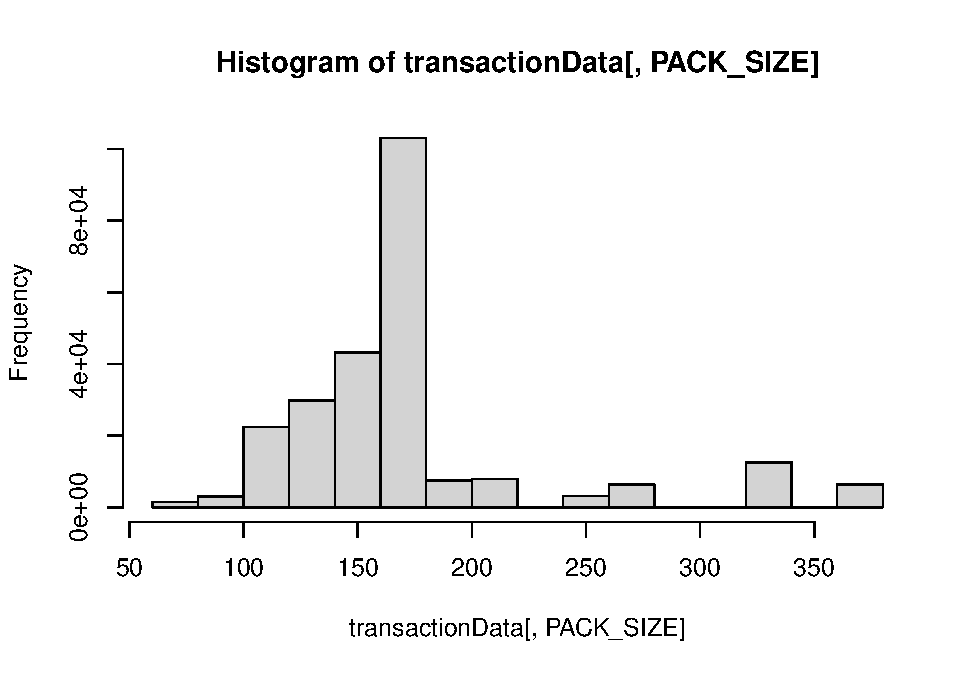
\includegraphics{InsideSherpa_Task1_files/figure-latex/unnamed-chunk-12-1.pdf}
Pack sizes created look reasonable. Now to create brands, we can use the
first word in PROD\_NAME to work out the brand name\ldots{}

\begin{Shaded}
\begin{Highlighting}[]
\DocumentationTok{\#\#\#\# Brands}
\CommentTok{\# Over to you! Create a column which contains the brand of the product, by extracting it from the product name.}
\DocumentationTok{\#\#\#\# Checking brands}
\CommentTok{\# Over to you! Check the results look reasonable.}
\NormalTok{transactionData}\SpecialCharTok{$}\NormalTok{BRAND }\OtherTok{\textless{}{-}} \FunctionTok{gsub}\NormalTok{(}\StringTok{"([A{-}Za{-}z]+).*"}\NormalTok{, }\StringTok{"}\SpecialCharTok{\textbackslash{}\textbackslash{}}\StringTok{1"}\NormalTok{, transactionData}\SpecialCharTok{$}\NormalTok{PROD\_NAME)}
\NormalTok{transactionData[, .N, by }\OtherTok{=}\NormalTok{ BRAND][}\FunctionTok{order}\NormalTok{(.N)]}
\end{Highlighting}
\end{Shaded}

\begin{verbatim}
##      BRAND     N
##     <char> <int>
## 1: Natural  6050
\end{verbatim}

Some of the brand names look like they are of the same brands - such as
RED and RRD, which are both Red Rock Deli chips. Let's combine these
together.

\begin{Shaded}
\begin{Highlighting}[]
\DocumentationTok{\#\#\#\# Clean brand names}
\NormalTok{transactionData[BRAND }\SpecialCharTok{==} \StringTok{"RED"}\NormalTok{, BRAND }\SpecialCharTok{:=} \StringTok{"RRD"}\NormalTok{]}
\CommentTok{\# Over to you! Add any additional brand adjustments you think may be required.}
\NormalTok{transactionData[BRAND }\SpecialCharTok{==} \StringTok{"SNBTS"}\NormalTok{, BRAND }\SpecialCharTok{:=} \StringTok{"SUNBITES"}\NormalTok{]}
\NormalTok{transactionData[BRAND }\SpecialCharTok{==} \StringTok{"INFZNS"}\NormalTok{, BRAND }\SpecialCharTok{:=} \StringTok{"INFUZIONS"}\NormalTok{]}
\NormalTok{transactionData[BRAND }\SpecialCharTok{==} \StringTok{"WW"}\NormalTok{, BRAND }\SpecialCharTok{:=} \StringTok{"WOOLWORTHS"}\NormalTok{]}
\NormalTok{transactionData[BRAND }\SpecialCharTok{==} \StringTok{"SMITH"}\NormalTok{, BRAND }\SpecialCharTok{:=} \StringTok{"SMITHS"}\NormalTok{]}
\NormalTok{transactionData[BRAND }\SpecialCharTok{==} \StringTok{"NCC"}\NormalTok{, BRAND }\SpecialCharTok{:=} \StringTok{"NATURAL"}\NormalTok{]}
\NormalTok{transactionData[BRAND }\SpecialCharTok{==} \StringTok{"DORITO"}\NormalTok{, BRAND }\SpecialCharTok{:=} \StringTok{"DORITOS"}\NormalTok{]}
\NormalTok{transactionData[BRAND }\SpecialCharTok{==} \StringTok{"GRAIN"}\NormalTok{, BRAND }\SpecialCharTok{:=} \StringTok{"GRNWVES"}\NormalTok{]}
\DocumentationTok{\#\#\#\# Check again}
\CommentTok{\# Over to you! Check the results look reasonable.}
\NormalTok{transactionData[, .N, by }\OtherTok{=}\NormalTok{ BRAND][}\FunctionTok{order}\NormalTok{(BRAND)]}
\end{Highlighting}
\end{Shaded}

\begin{verbatim}
##          BRAND     N
##         <char> <int>
##  1:     Burger  1564
##  2:        CCs  4551
##  3:    Cheetos  2927
##  4:   Cheezels  4603
##  5:       Cobs  9693
##  6:     Dorito  3185
##  7:    Doritos 22041
##  8:     French  1418
##  9:      Grain  6272
## 10:    GrnWves  1468
## 11:  Infuzions 11057
## 12:     Infzns  3144
## 13:     Kettle 41288
## 14:    NATURAL  1419
## 15:    Natural  6050
## 16:   Pringles 25102
## 17:        RRD 11894
## 18:        Red  4427
## 19:      Smith  2963
## 20:     Smiths 27390
## 21:      Snbts  1576
## 22:   Sunbites  1432
## 23:      Thins 14075
## 24:   Tostitos  9471
## 25:   Twisties  9454
## 26:   Tyrrells  6442
## 27: WOOLWORTHS 10320
## 28: Woolworths  1516
##          BRAND     N
\end{verbatim}

\subsubsection{Examining customer data}\label{examining-customer-data}

Now that we are happy with the transaction dataset, let's have a look at
the customer dataset.

\begin{Shaded}
\begin{Highlighting}[]
\DocumentationTok{\#\#\#\# Examining customer data}
\CommentTok{\# Over to you! Do some basic summaries of the dataset, including distributions on any key columns.}
\FunctionTok{summary}\NormalTok{(customerData)}
\end{Highlighting}
\end{Shaded}

\begin{verbatim}
##  LYLTY_CARD_NBR     LIFESTAGE         PREMIUM_CUSTOMER  
##  Min.   :   1000   Length:72637       Length:72637      
##  1st Qu.:  66202   Class :character   Class :character  
##  Median : 134040   Mode  :character   Mode  :character  
##  Mean   : 136186                                        
##  3rd Qu.: 203375                                        
##  Max.   :2373711
\end{verbatim}

\begin{Shaded}
\begin{Highlighting}[]
\DocumentationTok{\#\#\#\# Merge transaction data to customer data}
\NormalTok{data }\OtherTok{\textless{}{-}} \FunctionTok{merge}\NormalTok{(transactionData, customerData, }\AttributeTok{all.x =} \ConstantTok{TRUE}\NormalTok{)}
\end{Highlighting}
\end{Shaded}

As the number of rows in \texttt{data} is the same as that of
\texttt{transactionData}, we can be sure that no duplicates were
created. This is because we created \texttt{data} by setting
\texttt{all.x\ =\ TRUE} (in other words, a left join) which means take
all the rows in \texttt{transactionData} and find rows with matching
values in shared columns and then joining the details in these rows to
the \texttt{x} or the first mentioned table. Let's also check if some
customers were not matched on by checking for nulls.

\begin{Shaded}
\begin{Highlighting}[]
\CommentTok{\# Over to you! See if any transactions did not have a matched customer.}
\FunctionTok{apply}\NormalTok{(data, }\DecValTok{2}\NormalTok{, }\ControlFlowTok{function}\NormalTok{(x) }\FunctionTok{any}\NormalTok{(}\FunctionTok{is.na}\NormalTok{(x)))}
\end{Highlighting}
\end{Shaded}

\begin{verbatim}
##   LYLTY_CARD_NBR             DATE        STORE_NBR           TXN_ID 
##            FALSE            FALSE            FALSE            FALSE 
##         PROD_NBR        PROD_NAME         PROD_QTY        TOT_SALES 
##            FALSE            FALSE            FALSE            FALSE 
##        PACK_SIZE            BRAND        LIFESTAGE PREMIUM_CUSTOMER 
##            FALSE            FALSE            FALSE            FALSE
\end{verbatim}

Great, there are no nulls! So all our customers in the transaction data
has been accounted for in the customer dataset. Note that if you are
continuing with Task 2, you may want to retain this dataset which you
can write out as a csv

\begin{Shaded}
\begin{Highlighting}[]
\FunctionTok{fwrite}\NormalTok{(data, }\FunctionTok{paste0}\NormalTok{(filePath,}\StringTok{"QVI\_data.csv"}\NormalTok{))}
\end{Highlighting}
\end{Shaded}

Data exploration is now complete! \#\# Data analysis on customer
segments Now that the data is ready for analysis, we can define some
metrics of interest to the client: - Who spends the most on chips (total
sales), describing customers by lifestage and how premium their general
purchasing behaviour is - How many customers are in each segment - How
many chips are bought per customer by segment - What's the average chip
price by customer segment We could also ask our data team for more
information. Examples are: - The customer's total spend over the period
and total spend for each transaction to understand what proportion of
their grocery spend is on chips - Proportion of customers in each
customer segment overall to compare against the mix of customers who
purchase chips Let's start with calculating total sales by LIFESTAGE and
PREMIUM\_CUSTOMER and plotting the split by these segments to describe
which customer segment contribute most to chip sales.

\begin{Shaded}
\begin{Highlighting}[]
\DocumentationTok{\#\#\#\# Total sales by LIFESTAGE and PREMIUM\_CUSTOMER}
\CommentTok{\# Over to you! Calculate the summary of sales by those dimensions and create a plot.}
\NormalTok{total\_sales }\OtherTok{\textless{}{-}}\NormalTok{ data }\SpecialCharTok{\%\textgreater{}\%} \FunctionTok{group\_by}\NormalTok{(LIFESTAGE,PREMIUM\_CUSTOMER)}
\NormalTok{pf.total\_sales }\OtherTok{\textless{}{-}} \FunctionTok{summarise}\NormalTok{(total\_sales,}\AttributeTok{sales\_count=}\FunctionTok{sum}\NormalTok{(TOT\_SALES))}
\end{Highlighting}
\end{Shaded}

\begin{verbatim}
## `summarise()` has grouped output by 'LIFESTAGE'. You can override using the
## `.groups` argument.
\end{verbatim}

\begin{Shaded}
\begin{Highlighting}[]
\FunctionTok{summary}\NormalTok{(pf.total\_sales)}
\end{Highlighting}
\end{Shaded}

\begin{verbatim}
##   LIFESTAGE         PREMIUM_CUSTOMER    sales_count    
##  Length:21          Length:21          Min.   : 10761  
##  Class :character   Class :character   1st Qu.: 54444  
##  Mode  :character   Mode  :character   Median : 86338  
##                                        Mean   : 86023  
##                                        3rd Qu.:124649  
##                                        Max.   :156864
\end{verbatim}

\begin{Shaded}
\begin{Highlighting}[]
\DocumentationTok{\#\#\#\# Create plot}
\NormalTok{p }\OtherTok{\textless{}{-}} \FunctionTok{ggplot}\NormalTok{(pf.total\_sales) }\SpecialCharTok{+} \FunctionTok{geom\_mosaic}\NormalTok{(}\FunctionTok{aes}\NormalTok{(}\AttributeTok{weight =}\NormalTok{ sales\_count, }\AttributeTok{x =} \FunctionTok{product}\NormalTok{(PREMIUM\_CUSTOMER, LIFESTAGE),)) }\SpecialCharTok{+} \FunctionTok{labs}\NormalTok{(}\AttributeTok{x =} \StringTok{"Lifestage"}\NormalTok{, }\AttributeTok{y =} \StringTok{"Premium customer flag"}\NormalTok{, }\AttributeTok{title =} \StringTok{"Proportion of sales"}\NormalTok{) }\SpecialCharTok{+} \FunctionTok{theme}\NormalTok{(}\AttributeTok{axis.text.x =} \FunctionTok{element\_text}\NormalTok{(}\AttributeTok{angle =} \DecValTok{90}\NormalTok{, }\AttributeTok{vjust =} \FloatTok{0.5}\NormalTok{)) }
\NormalTok{p }\SpecialCharTok{+}\FunctionTok{geom\_text}\NormalTok{(}\AttributeTok{data =} \FunctionTok{ggplot\_build}\NormalTok{(p)}\SpecialCharTok{$}\NormalTok{data[[}\DecValTok{1}\NormalTok{]], }\FunctionTok{aes}\NormalTok{(}\AttributeTok{x =}\NormalTok{ (xmin }\SpecialCharTok{+}\NormalTok{ xmax)}\SpecialCharTok{/}\DecValTok{2}\NormalTok{ , }\AttributeTok{y =}\NormalTok{ (ymin }\SpecialCharTok{+}\NormalTok{ ymax)}\SpecialCharTok{/}\DecValTok{2}\NormalTok{, }\AttributeTok{label =} \FunctionTok{as.character}\NormalTok{(}\FunctionTok{paste}\NormalTok{(}\FunctionTok{round}\NormalTok{(.wt}\SpecialCharTok{/}\FunctionTok{sum}\NormalTok{(.wt),}\DecValTok{3}\NormalTok{)}\SpecialCharTok{*}\DecValTok{100}\NormalTok{, }\StringTok{\textquotesingle{}\%\textquotesingle{}}\NormalTok{))), }\AttributeTok{inherit.aes =}\NormalTok{ F)}
\end{Highlighting}
\end{Shaded}

\begin{verbatim}
## Warning: `unite_()` was deprecated in tidyr 1.2.0.
## i Please use `unite()` instead.
## i The deprecated feature was likely used in the ggmosaic package.
##   Please report the issue at <https://github.com/haleyjeppson/ggmosaic>.
## This warning is displayed once every 8 hours.
## Call `lifecycle::last_lifecycle_warnings()` to see where this warning was
## generated.
\end{verbatim}

\begin{center}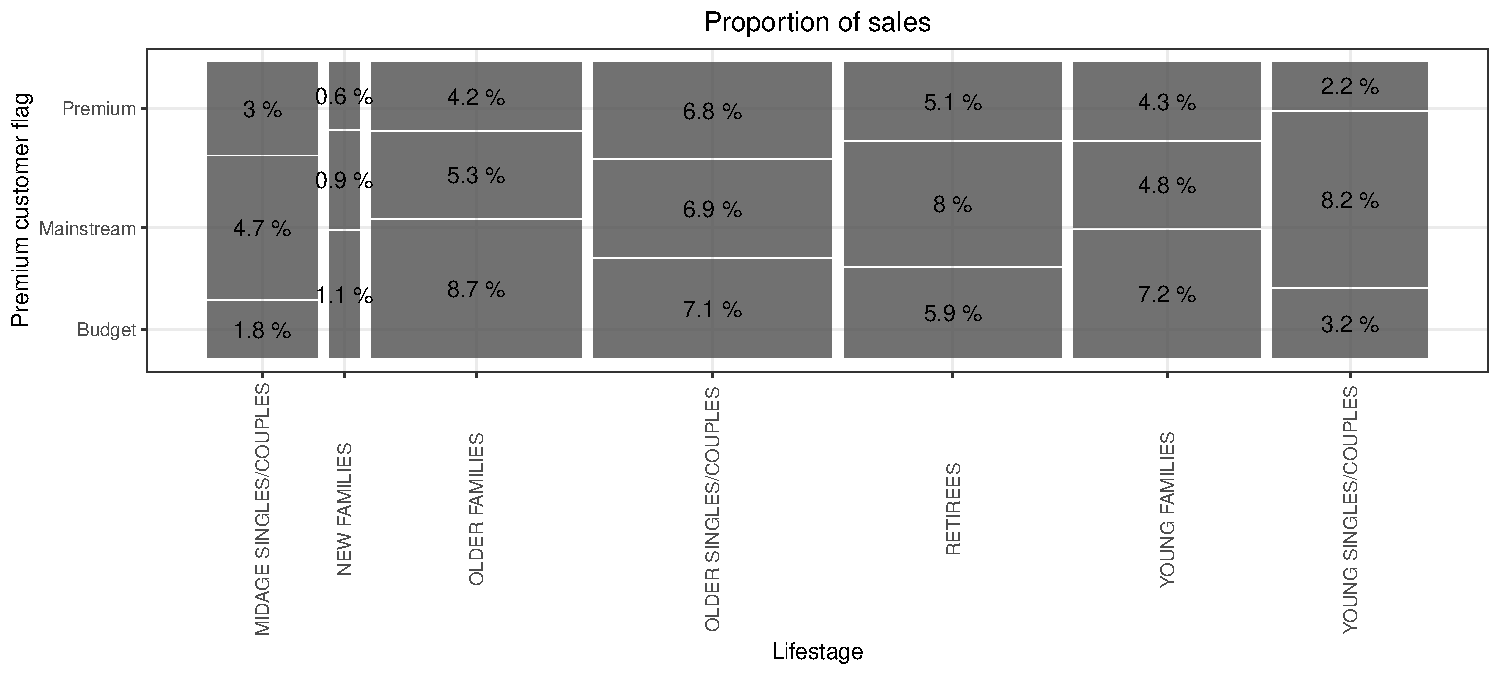
\includegraphics{InsideSherpa_Task1_files/figure-latex/unnamed-chunk-14-1} \end{center}

Sales are coming mainly from Budget - older families, Mainstream - young
singles/couples, and Mainstream - retirees Let's see if the higher sales
are due to there being more customers who buy chips.

\begin{Shaded}
\begin{Highlighting}[]
\DocumentationTok{\#\#\#\# Number of customers by LIFESTAGE and PREMIUM\_CUSTOMER}
\CommentTok{\# Over to you! Calculate the summary of number of customers by those dimensions and create a plot.}
\NormalTok{total\_sales }\OtherTok{\textless{}{-}}\NormalTok{ data }\SpecialCharTok{\%\textgreater{}\%} \FunctionTok{group\_by}\NormalTok{(LIFESTAGE,PREMIUM\_CUSTOMER)}
\NormalTok{no\_of\_customers }\OtherTok{\textless{}{-}} \FunctionTok{summarise}\NormalTok{(total\_sales,}\AttributeTok{customer\_count =} \FunctionTok{length}\NormalTok{(}\FunctionTok{unique}\NormalTok{(LYLTY\_CARD\_NBR))) }
\end{Highlighting}
\end{Shaded}

\begin{verbatim}
## `summarise()` has grouped output by 'LIFESTAGE'. You can override using the
## `.groups` argument.
\end{verbatim}

\begin{Shaded}
\begin{Highlighting}[]
\FunctionTok{summary}\NormalTok{(no\_of\_customers)}
\end{Highlighting}
\end{Shaded}

\begin{verbatim}
##   LIFESTAGE         PREMIUM_CUSTOMER   customer_count
##  Length:21          Length:21          Min.   : 575  
##  Class :character   Class :character   1st Qu.:2369  
##  Mode  :character   Mode  :character   Median :3298  
##                                        Mean   :3395  
##                                        3rd Qu.:4611  
##                                        Max.   :7917
\end{verbatim}

\begin{Shaded}
\begin{Highlighting}[]
\DocumentationTok{\#\#\#\# Create plot}
\NormalTok{p }\OtherTok{\textless{}{-}} \FunctionTok{ggplot}\NormalTok{(}\AttributeTok{data =}\NormalTok{ no\_of\_customers) }\SpecialCharTok{+} \FunctionTok{geom\_mosaic}\NormalTok{(}\FunctionTok{aes}\NormalTok{(}\AttributeTok{weight =}\NormalTok{ customer\_count, }\AttributeTok{x =} \FunctionTok{product}\NormalTok{(PREMIUM\_CUSTOMER, LIFESTAGE))) }\SpecialCharTok{+} \FunctionTok{labs}\NormalTok{(}\AttributeTok{x =} \StringTok{"Lifestage"}\NormalTok{, }\AttributeTok{y =} \StringTok{"Premium customer flag"}\NormalTok{, }\AttributeTok{title =} \StringTok{"Proportion of customers"}\NormalTok{) }\SpecialCharTok{+} \FunctionTok{theme}\NormalTok{(}\AttributeTok{axis.text.x =} \FunctionTok{element\_text}\NormalTok{(}\AttributeTok{angle =} \DecValTok{90}\NormalTok{, }\AttributeTok{vjust =} \FloatTok{0.5}\NormalTok{))}\SpecialCharTok{+} \FunctionTok{geom\_text}\NormalTok{(}\AttributeTok{data =} \FunctionTok{ggplot\_build}\NormalTok{(p)}\SpecialCharTok{$}\NormalTok{data[[}\DecValTok{1}\NormalTok{]], }\FunctionTok{aes}\NormalTok{(}\AttributeTok{x =}\NormalTok{ (xmin }\SpecialCharTok{+}\NormalTok{ xmax)}\SpecialCharTok{/}\DecValTok{2}\NormalTok{ , }\AttributeTok{y =}\NormalTok{ (ymin }\SpecialCharTok{+}\NormalTok{ ymax)}\SpecialCharTok{/}\DecValTok{2}\NormalTok{, }\AttributeTok{label =} \FunctionTok{as.character}\NormalTok{(}\FunctionTok{paste}\NormalTok{(}\FunctionTok{round}\NormalTok{(.wt}\SpecialCharTok{/}\FunctionTok{sum}\NormalTok{(.wt),}\DecValTok{3}\NormalTok{)}\SpecialCharTok{*}\DecValTok{100}\NormalTok{, }\StringTok{\textquotesingle{}\%\textquotesingle{}}\NormalTok{))))}
\NormalTok{p}
\end{Highlighting}
\end{Shaded}

\begin{center}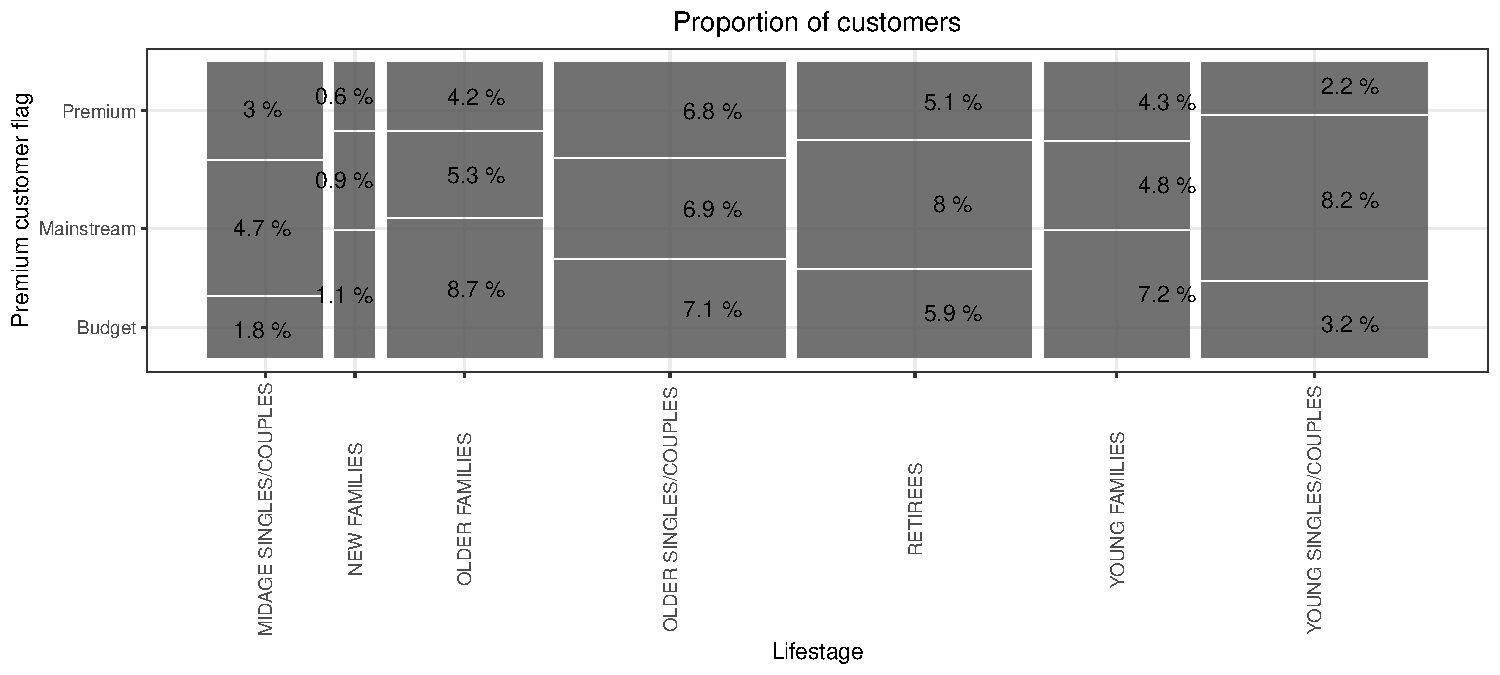
\includegraphics{InsideSherpa_Task1_files/figure-latex/unnamed-chunk-15-1} \end{center}

There are more Mainstream - young singles/couples and Mainstream -
retirees who buy chips. This contributes to there being more sales to
these customer segments but this is not a major driver for the Budget -
Older families segment. Higher sales may also be driven by more units of
chips being bought per customer. Let's have a look at this next.

\begin{Shaded}
\begin{Highlighting}[]
\DocumentationTok{\#\#\#\# Average number of units per customer by LIFESTAGE and PREMIUM\_CUSTOMER}
\CommentTok{\# Over to you! Calculate and plot the average number of units per customer by those two dimensions.}
\NormalTok{total\_sales\_1 }\OtherTok{\textless{}{-}}\NormalTok{data }\SpecialCharTok{\%\textgreater{}\%} \FunctionTok{group\_by}\NormalTok{(LIFESTAGE,PREMIUM\_CUSTOMER)}
\NormalTok{units }\OtherTok{\textless{}{-}}  \FunctionTok{summarise}\NormalTok{(total\_sales\_1, }\AttributeTok{units\_count =}\NormalTok{ (}\FunctionTok{sum}\NormalTok{(PROD\_QTY)}\SpecialCharTok{/}\FunctionTok{uniqueN}\NormalTok{(LYLTY\_CARD\_NBR)))}
\end{Highlighting}
\end{Shaded}

\begin{verbatim}
## `summarise()` has grouped output by 'LIFESTAGE'. You can override using the
## `.groups` argument.
\end{verbatim}

\begin{Shaded}
\begin{Highlighting}[]
\FunctionTok{summary}\NormalTok{(units)}
\end{Highlighting}
\end{Shaded}

\begin{verbatim}
##   LIFESTAGE         PREMIUM_CUSTOMER    units_count   
##  Length:21          Length:21          Min.   :4.250  
##  Class :character   Class :character   1st Qu.:4.892  
##  Mode  :character   Mode  :character   Median :6.142  
##                                        Mean   :6.583  
##                                        3rd Qu.:8.638  
##                                        Max.   :9.255
\end{verbatim}

\begin{Shaded}
\begin{Highlighting}[]
\DocumentationTok{\#\#\#create plot}
\FunctionTok{ggplot}\NormalTok{(}\AttributeTok{data =}\NormalTok{ units, }\FunctionTok{aes}\NormalTok{(}\AttributeTok{weight =}\NormalTok{ units\_count, }\AttributeTok{x =}\NormalTok{ LIFESTAGE, }\AttributeTok{fill =}\NormalTok{ PREMIUM\_CUSTOMER)) }\SpecialCharTok{+} \FunctionTok{geom\_bar}\NormalTok{(}\AttributeTok{position =} \FunctionTok{position\_dodge}\NormalTok{()) }\SpecialCharTok{+}
\FunctionTok{labs}\NormalTok{(}\AttributeTok{x =} \StringTok{"Lifestage"}\NormalTok{, }\AttributeTok{y =} \StringTok{"Avg units per transaction"}\NormalTok{, }\AttributeTok{title =} \StringTok{"Units per customer"}\NormalTok{) }\SpecialCharTok{+} \FunctionTok{theme}\NormalTok{(}\AttributeTok{axis.text.x =} \FunctionTok{element\_text}\NormalTok{(}\AttributeTok{angle =} \DecValTok{90}\NormalTok{, }\AttributeTok{vjust =} \FloatTok{0.5}\NormalTok{))}
\end{Highlighting}
\end{Shaded}

\begin{center}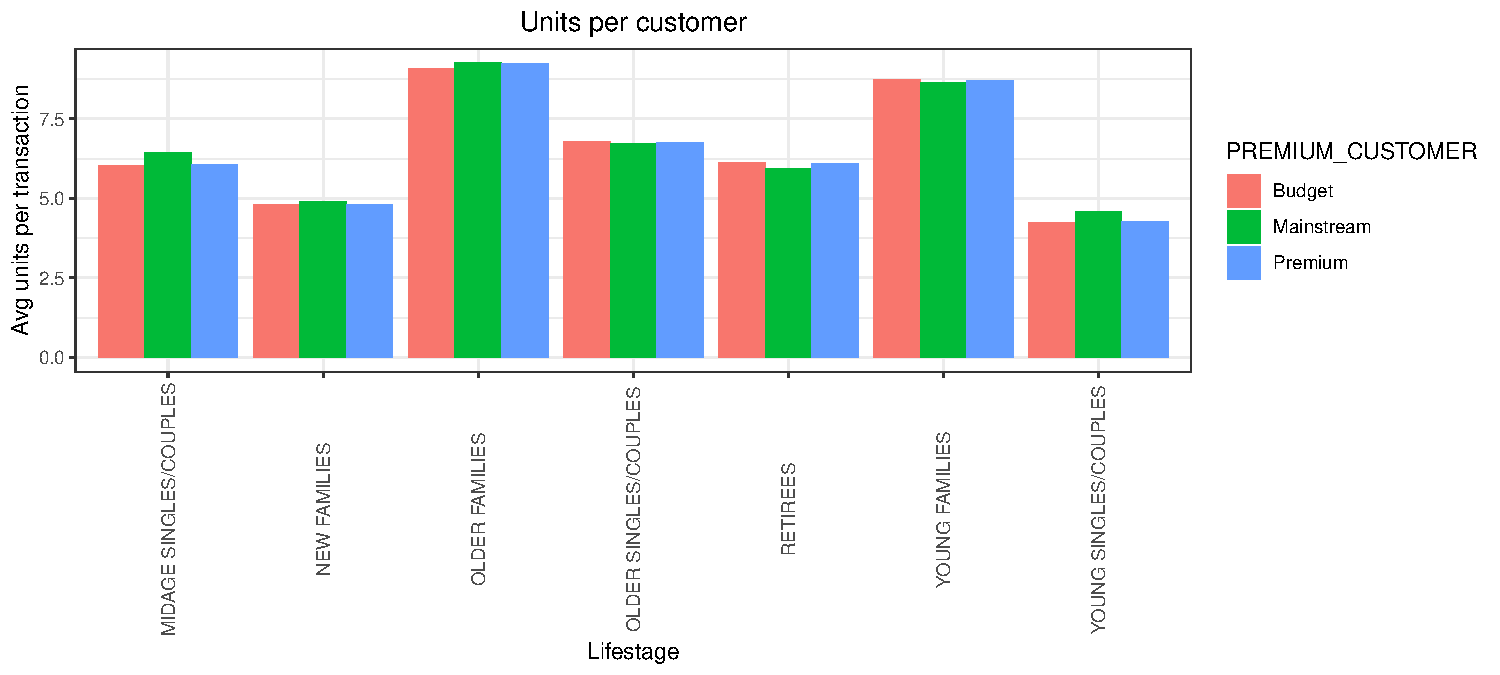
\includegraphics{InsideSherpa_Task1_files/figure-latex/unnamed-chunk-16-1} \end{center}

Older families and young families in general buy more chips per customer
Let's also investigate the average price per unit chips bought for each
customer segment as this is also a driver of total sales.

\begin{Shaded}
\begin{Highlighting}[]
\DocumentationTok{\#\#\#\# Average price per unit by LIFESTAGE and PREMIUM\_CUSTOMER}
\CommentTok{\# Over to you! Calculate and plot the average price per unit sold (average sale price) by those two customer dimensions.}
\end{Highlighting}
\end{Shaded}

Mainstream midage and young singles and couples are more willing to pay
more per packet of chips compared to their budget and premium
counterparts. This may be due to premium shoppers being more likely to
buy healthy snacks and when they buy chips, this is mainly for
entertainment purposes rather than their own consumption. This is also
supported by there being fewer premium midage and young singles and
couples buying chips compared to their mainstream counterparts. As the
difference in average price per unit isn't large, we can check if this
difference is statistically different.

\begin{Shaded}
\begin{Highlighting}[]
\DocumentationTok{\#\#\#\# Perform an independent t{-}test between mainstream vs premium and budget midage and}
\DocumentationTok{\#\#\#\# young singles and couples}
\CommentTok{\# Over to you! Perform a t{-}test to see if the difference is significant.}
\NormalTok{pricePerUnit }\OtherTok{\textless{}{-}}\NormalTok{ data[, price }\SpecialCharTok{:=}\NormalTok{ TOT\_SALES}\SpecialCharTok{/}\NormalTok{PROD\_QTY]}
\FunctionTok{t.test}\NormalTok{(data[LIFESTAGE }\SpecialCharTok{\%in\%} \FunctionTok{c}\NormalTok{(}\StringTok{"YOUNG SINGLES/COUPLES"}\NormalTok{, }\StringTok{"MIDAGE SINGLES/COUPLES"}\NormalTok{) }\SpecialCharTok{\&}\NormalTok{ PREMIUM\_CUSTOMER }\SpecialCharTok{==} \StringTok{"Mainstream"}\NormalTok{, price], data[LIFESTAGE }\SpecialCharTok{\%in\%} \FunctionTok{c}\NormalTok{(}\StringTok{"YOUNG SINGLES/COUPLES"}\NormalTok{, }\StringTok{"MIDAGE SINGLES/COUPLES"}\NormalTok{) }\SpecialCharTok{\&}\NormalTok{ PREMIUM\_CUSTOMER }\SpecialCharTok{!=} \StringTok{"Mainstream"}\NormalTok{, price], }\AttributeTok{alternative =} \StringTok{"greater"}\NormalTok{ )}
\end{Highlighting}
\end{Shaded}

\begin{verbatim}
##
## Welch Two Sample t-test
##
## data: data[LIFESTAGE %in% c("YOUNG SINGLES/COUPLES", "MIDAGE
SINGLES/COUPLES") & PREMIUM_CUSTOMER == "Mainstream", price] and data[LIFESTAGE
%in% c("YOUNG SINGLES/COUPLES", "MIDAGE SINGLES/COUPLES") & PREMIUM_CUSTOMER !=
"Mainstream", price]
## t = 37.624, df = 54791, p-value < 2.2e-16
## alternative hypothesis: true difference in means is greater than 0
## 95 percent confidence interval:
## 0.3187234 Inf
## sample estimates:
## mean of x mean of y
## 4.039786 3.706491
\end{verbatim}

The t-test results in a p-value of XXXXXXX, i.e.~the unit price for
mainstream, young and mid-age singles and couples {[}ARE / ARE NOT{]}
significantly higher than that of budget or premium, young and midage
singles and couples. \#\# Deep dive into specific customer segments for
insights We have found quite a few interesting insights that we can dive
deeper into. We might want to target customer segments that contribute
the most to sales to retain them or further increase sales. Let's look
at Mainstream - young singles/couples. For instance, let's find out if
they tend to buy a particular brand of chips.

\begin{Shaded}
\begin{Highlighting}[]
\DocumentationTok{\#\#\#\# Deep dive into Mainstream, young singles/couples}
\CommentTok{\# Over to you! Work out of there are brands that these two customer segments prefer more than others. You could use a technique called affinity analysis or a{-}priori analysis (or any other method if you prefer)}
\end{Highlighting}
\end{Shaded}

We can see that : {[}INSIGHTS{]} Let's also find out if our target
segment tends to buy larger packs of chips.

\begin{Shaded}
\begin{Highlighting}[]
\DocumentationTok{\#\#\#\# Preferred pack size compared to the rest of the population}
\CommentTok{\# Over to you! Do the same for pack size.}
\end{Highlighting}
\end{Shaded}

{[}INSIGHTS{]}

\end{document}
